\chapter{Descrierea Aplicației TickLy}
\label{sec:descriere-aplicatie}

Sistemul TickLy este o platformă de tip Help Desk concepută pentru gestionarea incidentelor și solicitărilor de suport. Aplicația oferă funcționalități de bază pentru managementul fluxului de lucru și analiză avansată a datelor prin module de raportare.

\section{Funcționalități Principale}
Aplicația permite realizarea următoarelor operațiuni:
\begin{itemize}
    \item \textbf{Management Tichete (CRU):} Utilizatorii pot crea, vizualiza si actualiza. Fiecare tichet include detalii despre prioritate, status, departament și subiectul vizat.
    \item \textbf{Comunicare și Colaborare:} Sistem de comentarii integrat pentru clienți și agenți, permițând monitorizarea istoricului conversației și jurnalizarea acțiunilor de audit în \textit{Ticket History}.
    \item \textbf{Model distribuit:} Agentii cand se conecteaza la aplicatie, pot vedea toate ticketele din sistem; fiecare client poate doar tichetele create de el; Agent poate vedea toate tichetele.
\end{itemize}

\begin{figure}[H]
    \centering
    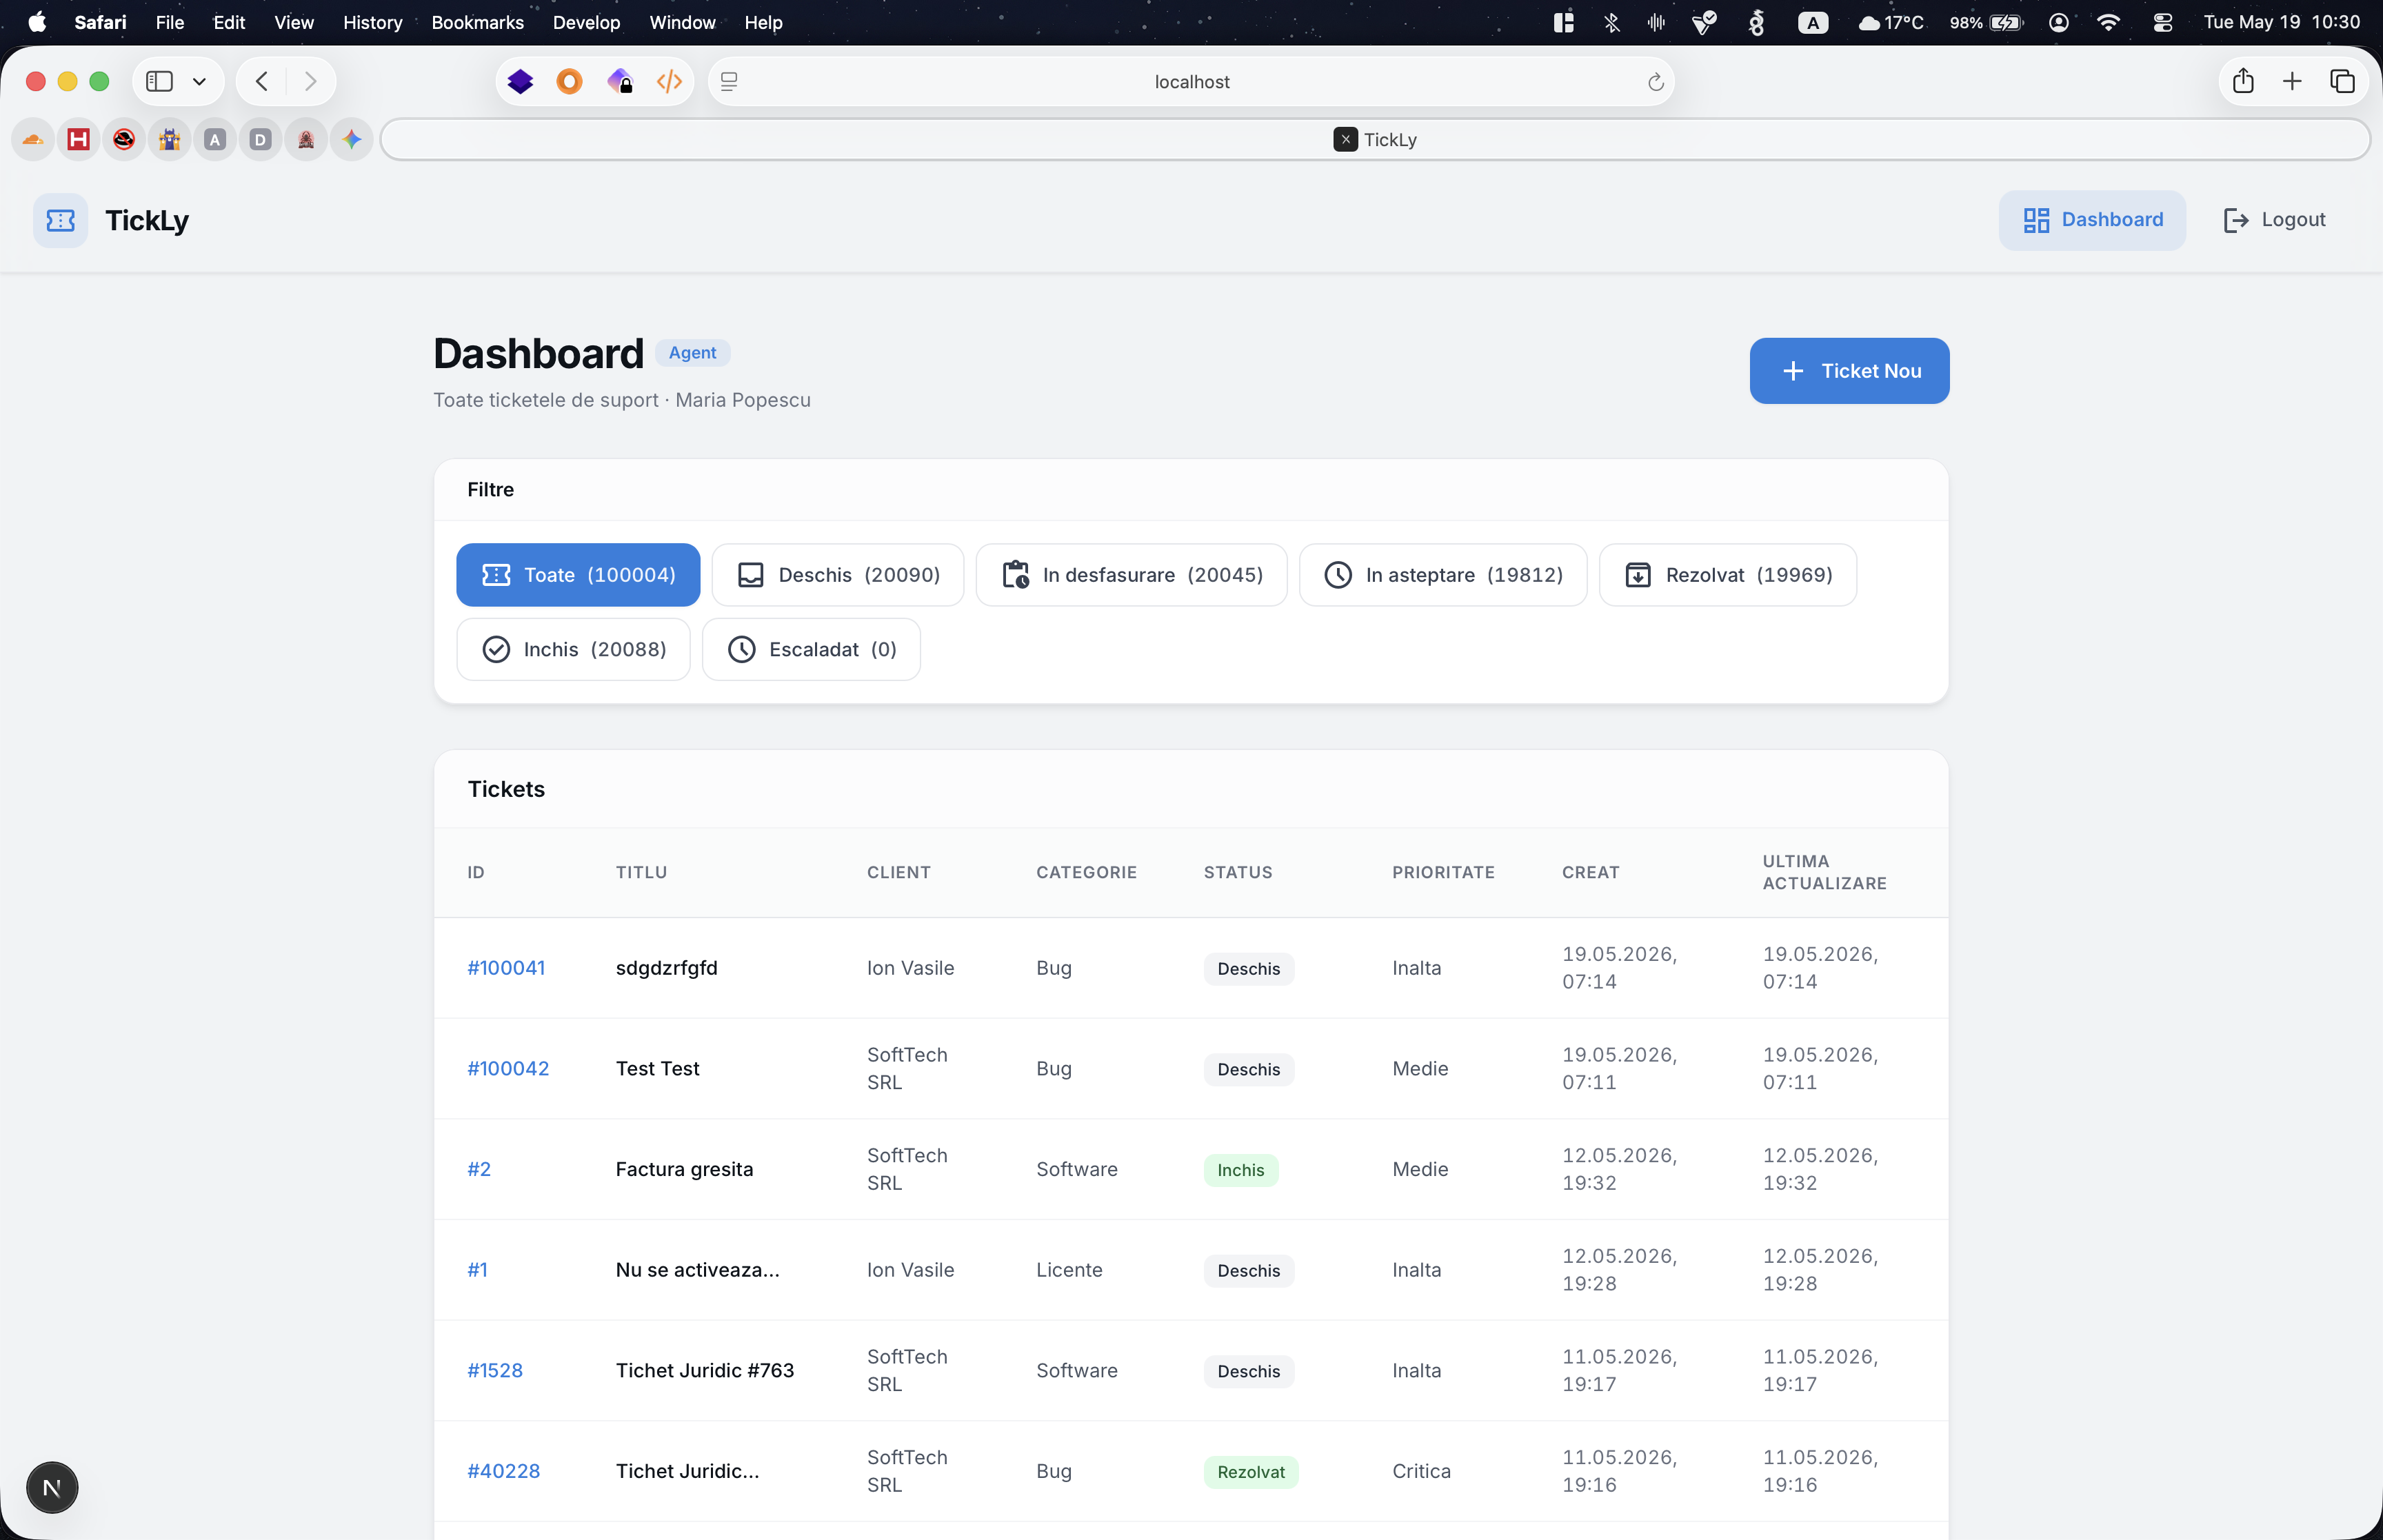
\includegraphics[width=0.6\textwidth]{./assets/app/global_module.png}
    \caption{Global Model - Agent View}
    \label{fig:dashboard}
\end{figure}

\begin{figure}[H]
    \centering
    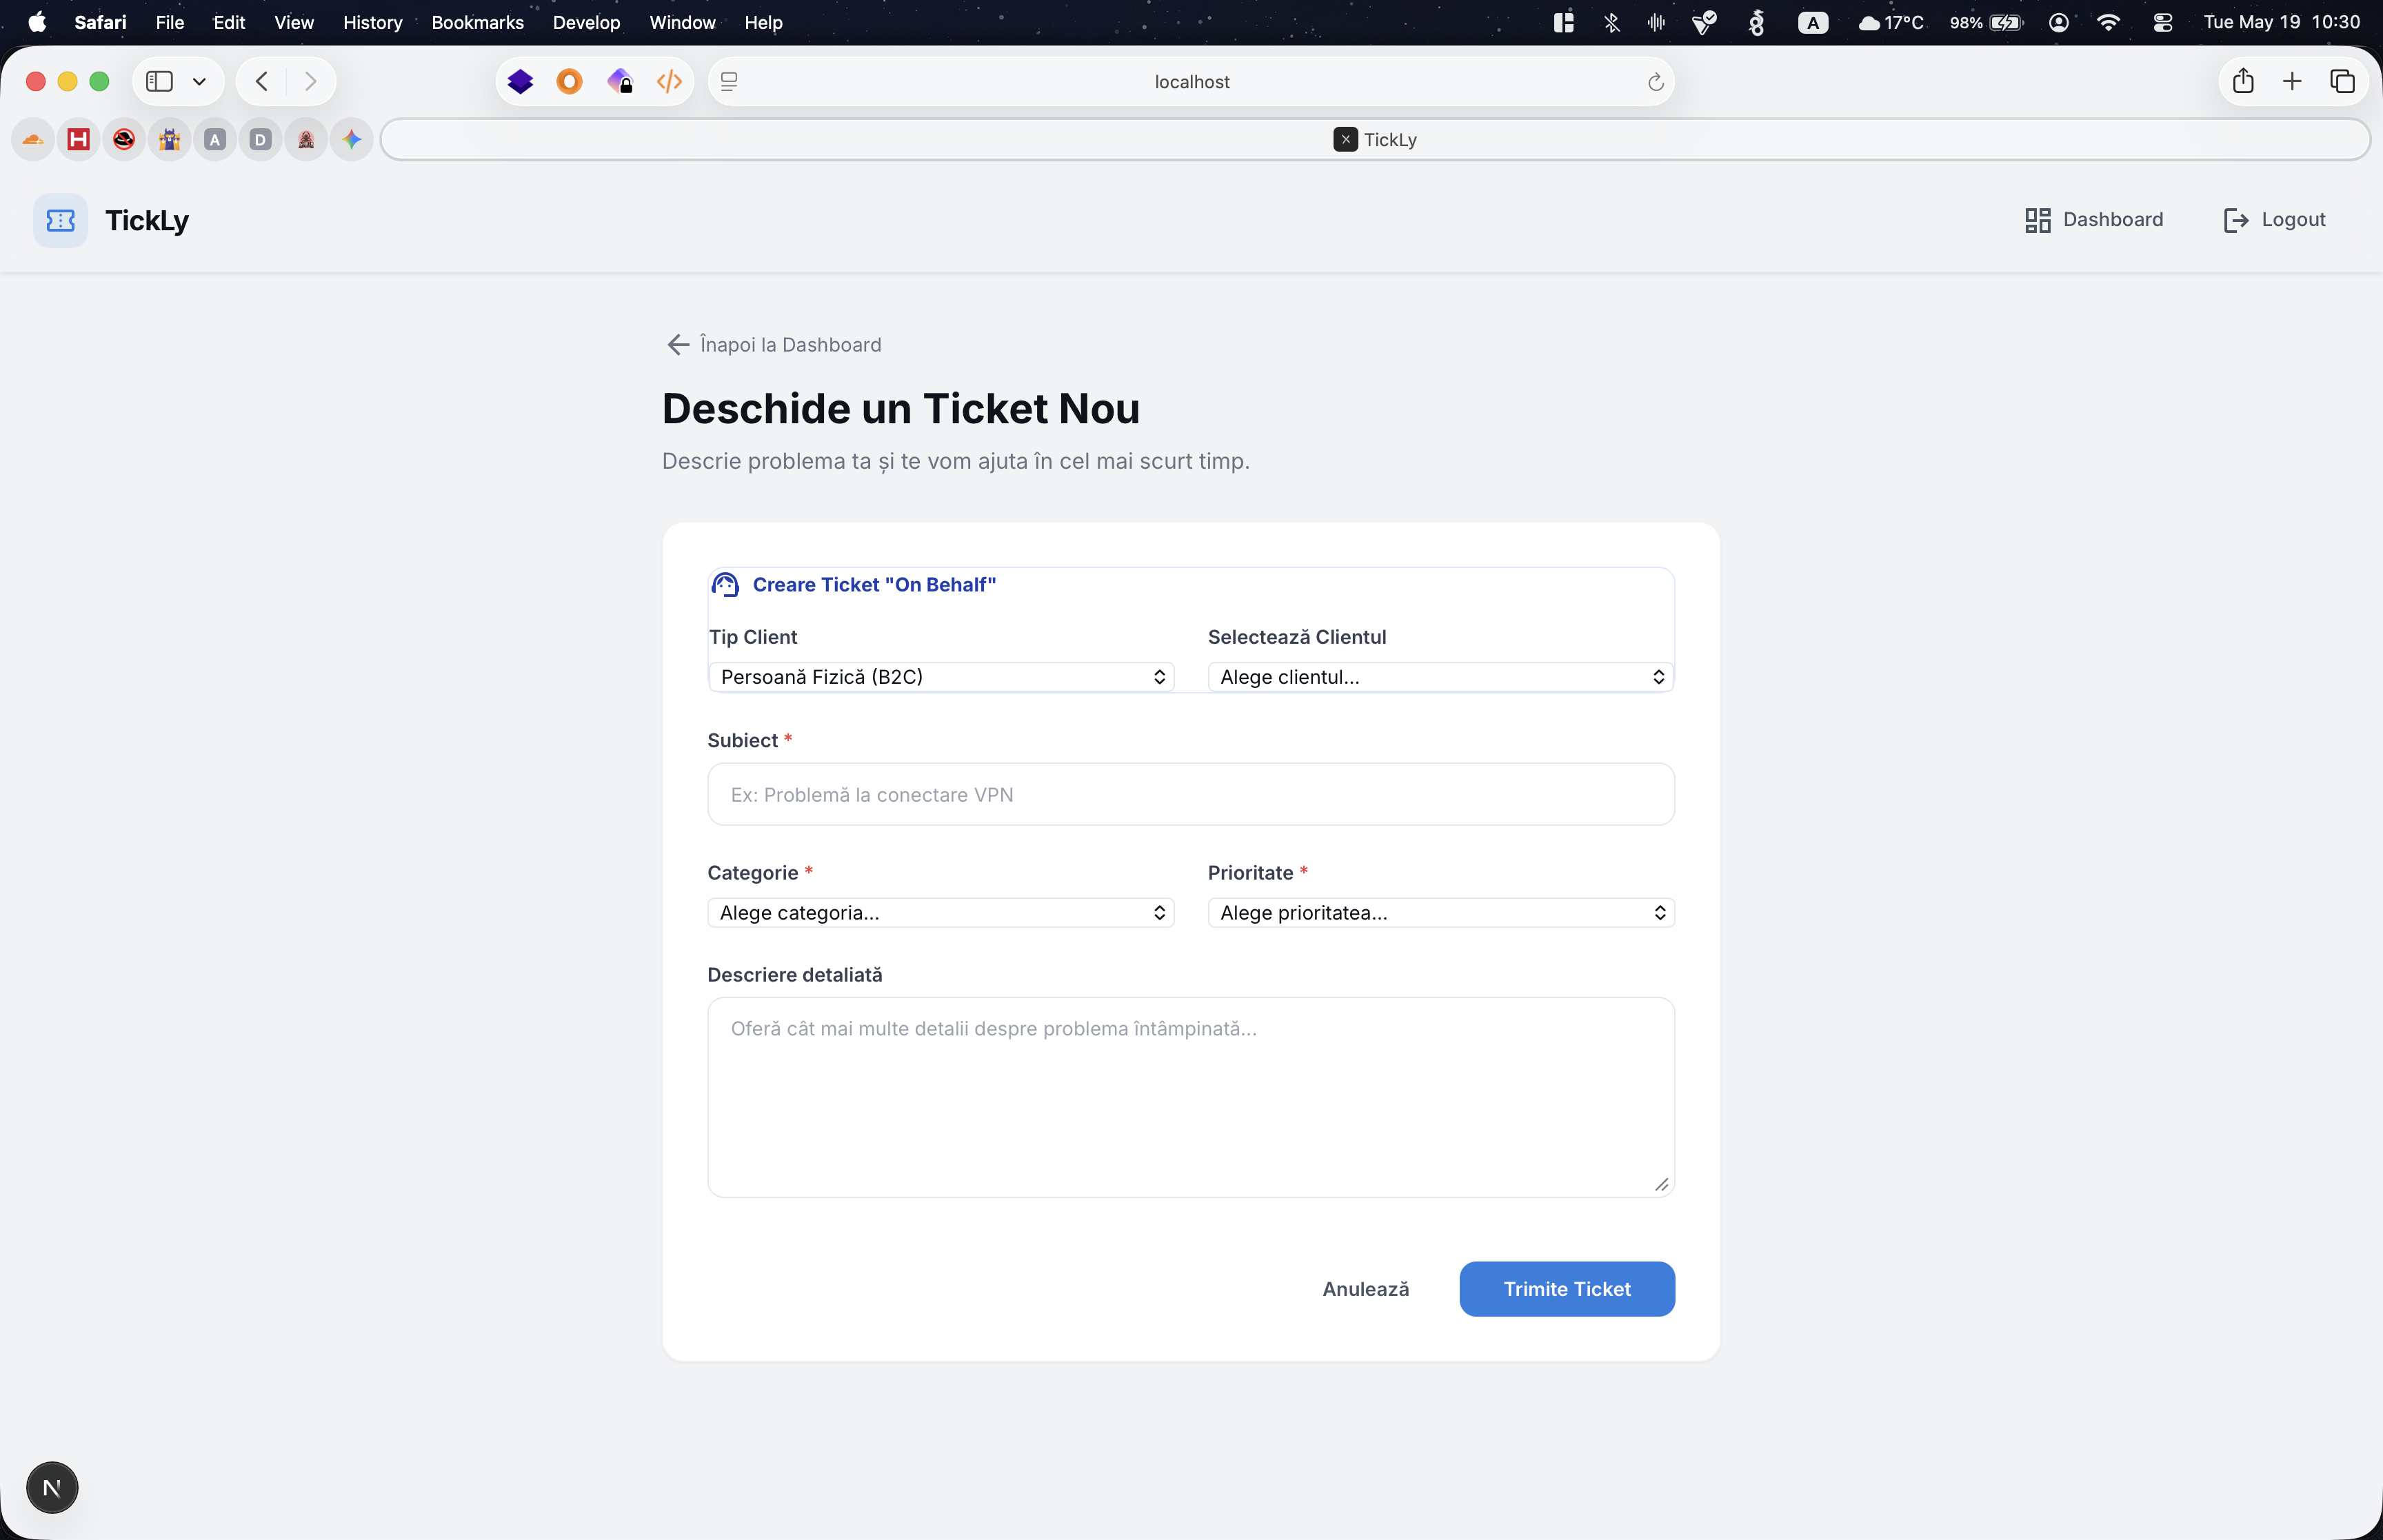
\includegraphics[width=0.6\textwidth]{./assets/app/agent_view.png}
    \caption{Global Model - New ticket Agent}
    \label{fig:newtkt_agent}
\end{figure}

\begin{figure}[H]
    \centering
    \begin{subfigure}[b]{0.48\textwidth}
        \centering
        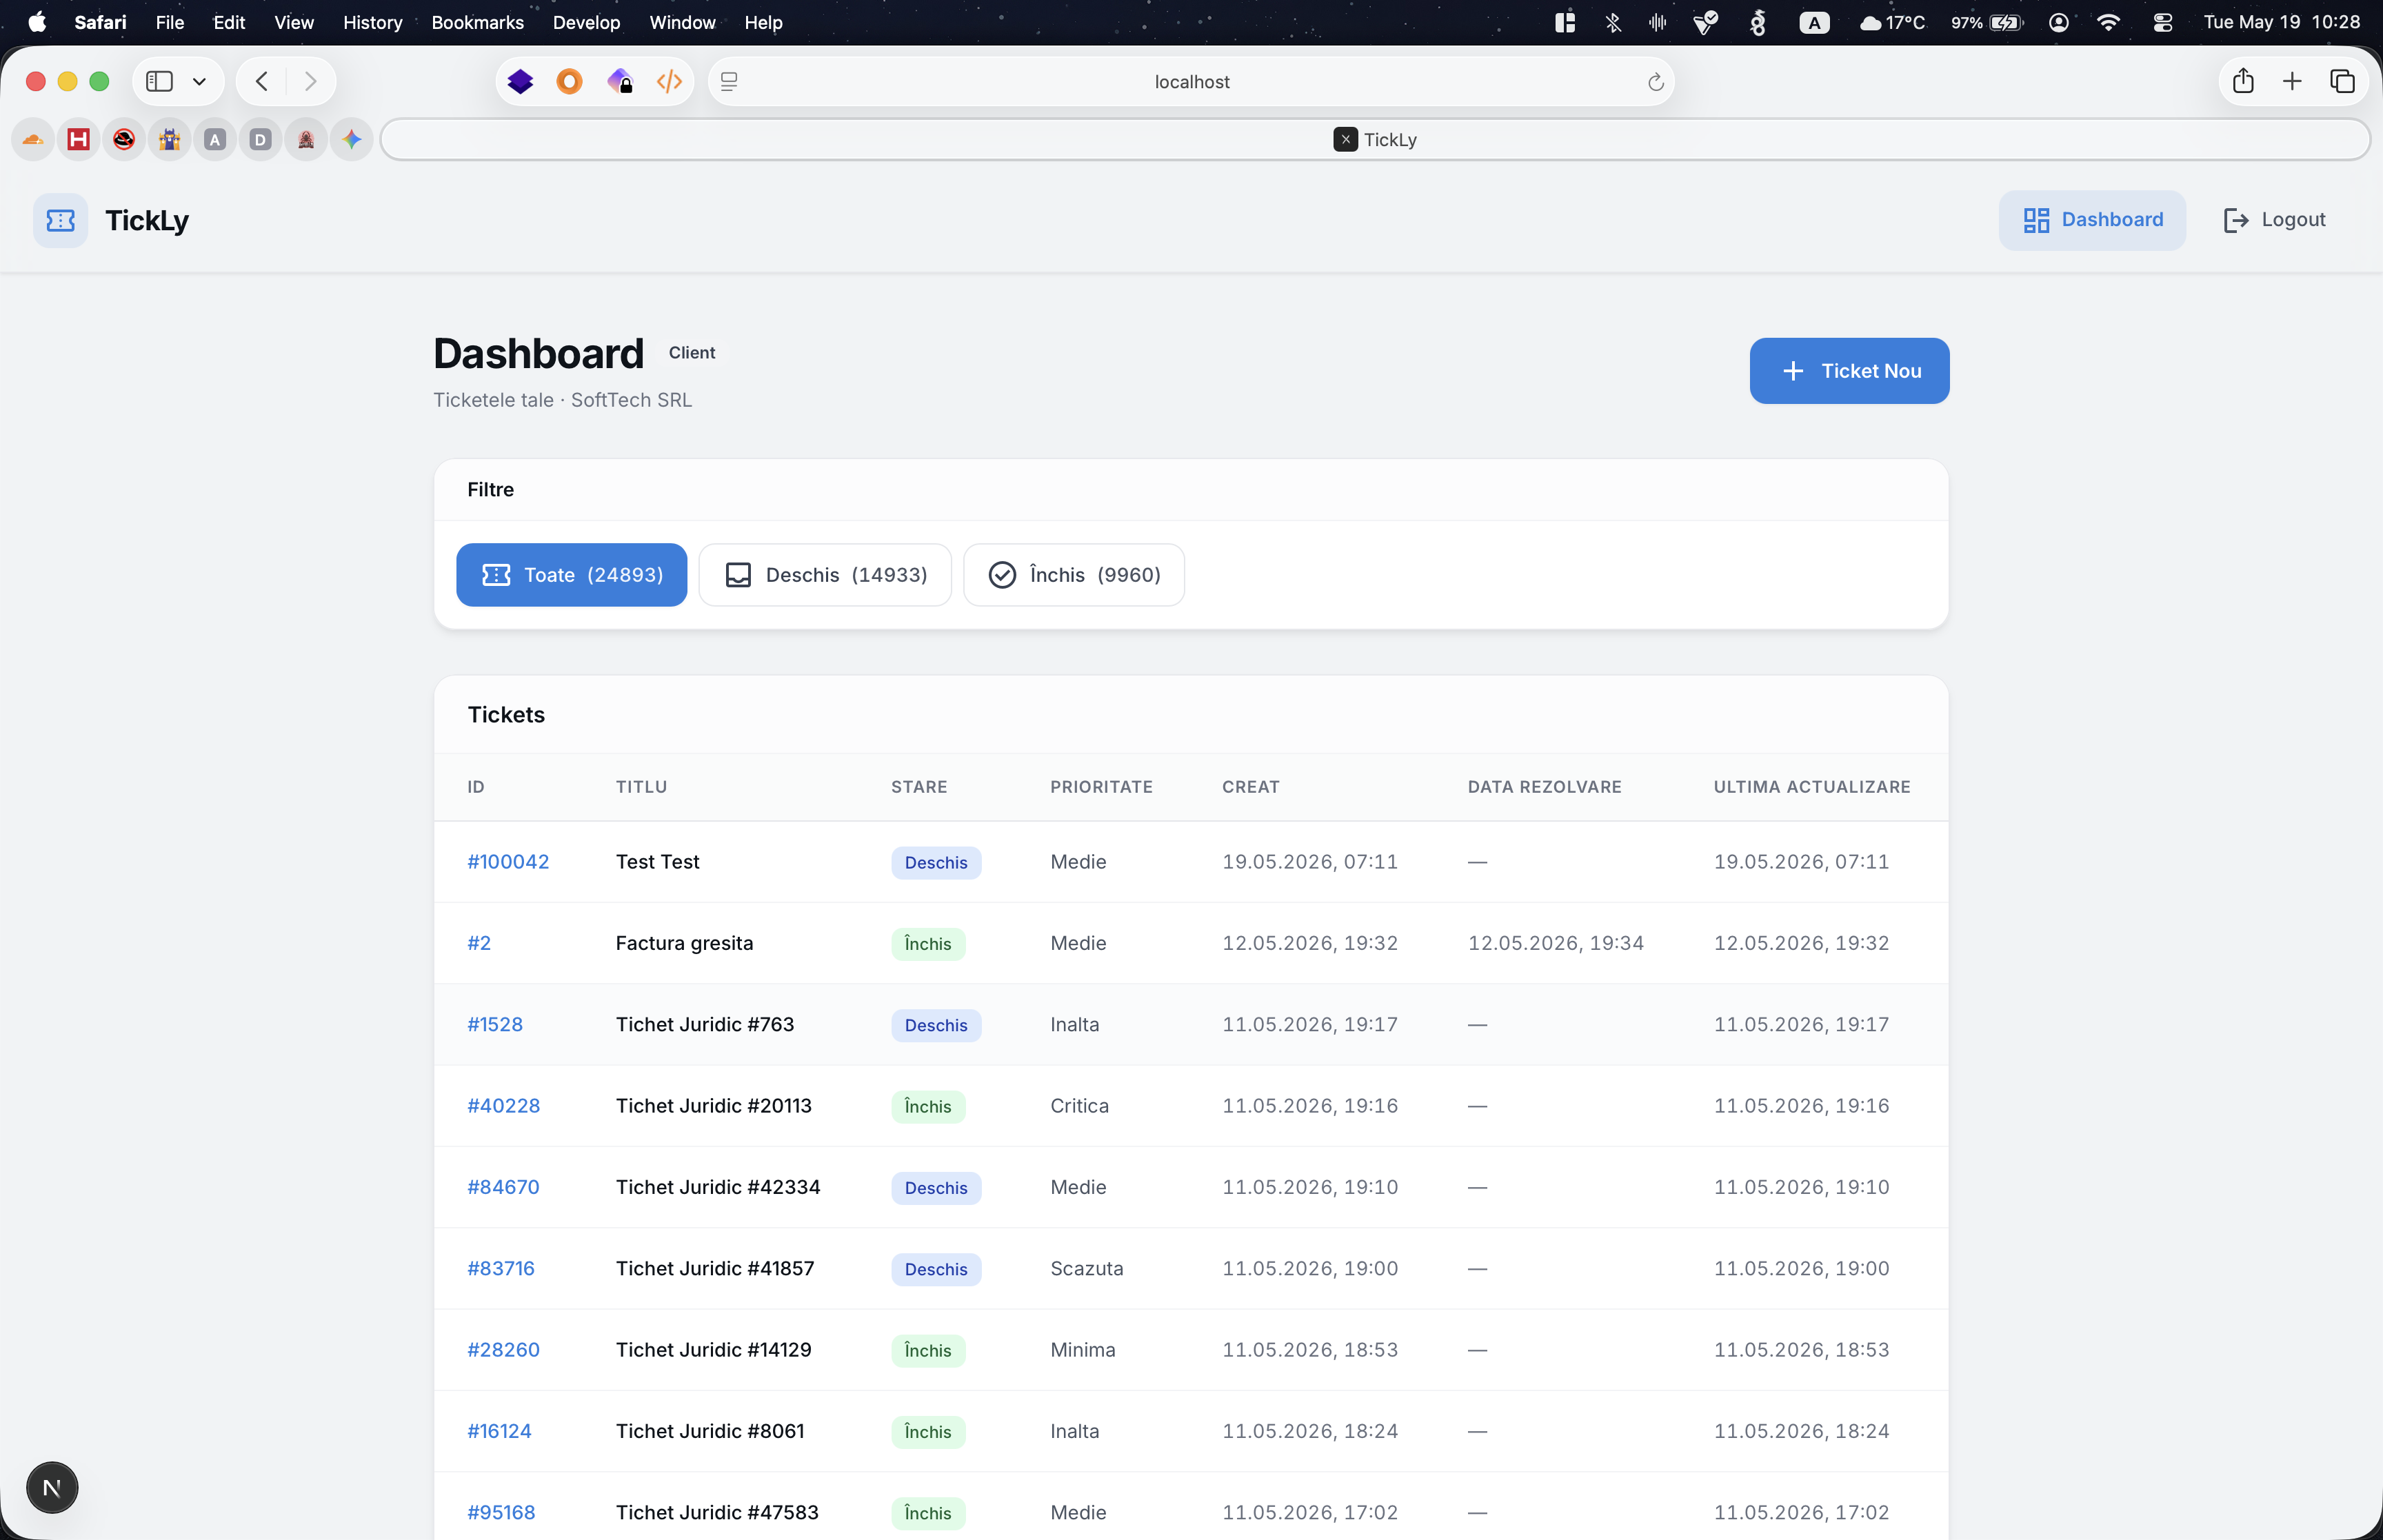
\includegraphics[width=\textwidth]{./assets/app/b2b_module_pt1.png}
        \label{fig:local_view_b2b_1}
    \end{subfigure}
    \hfill
    \begin{subfigure}[b]{0.48\textwidth}
        \centering
        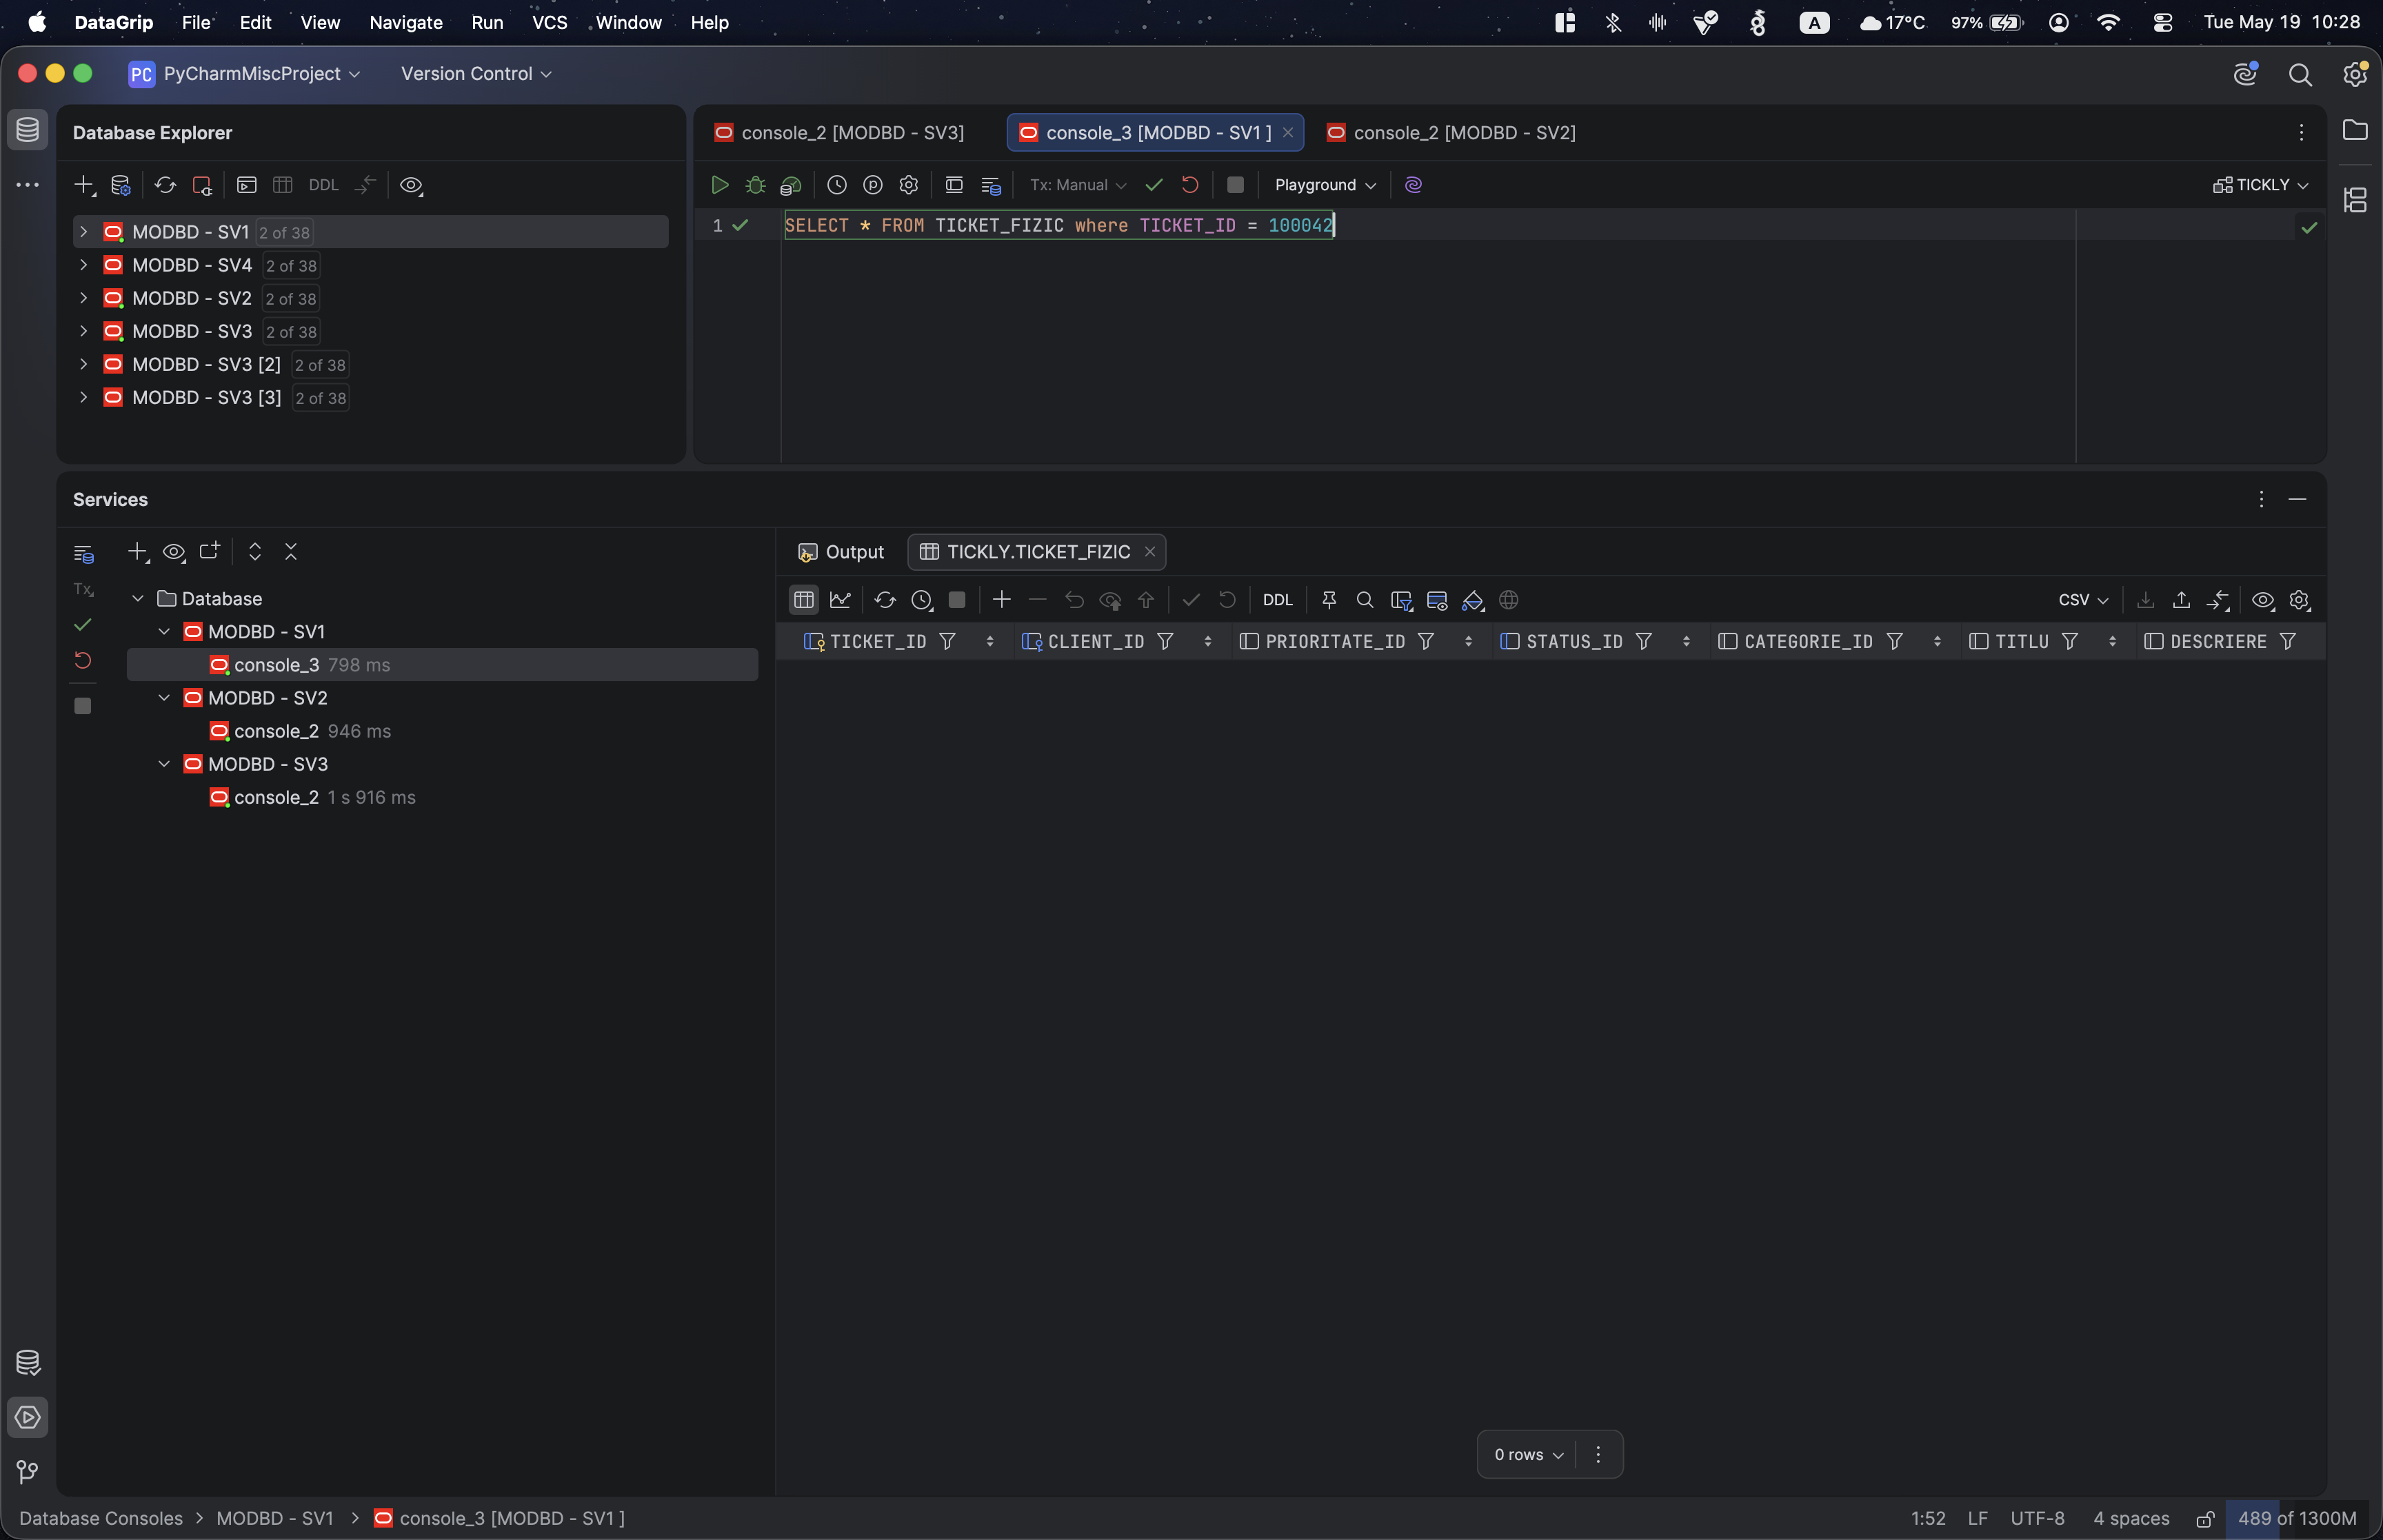
\includegraphics[width=\textwidth]{./assets/app/b2b_module_pt2.png}
        \label{fig:local_view_b2b_2}
    \end{subfigure}
    
    \caption{Local Model B2B}
    \label{fig:dashboard}
\end{figure}

\begin{figure}[H]
    \centering
    \begin{subfigure}[b]{0.48\textwidth}
        \centering
        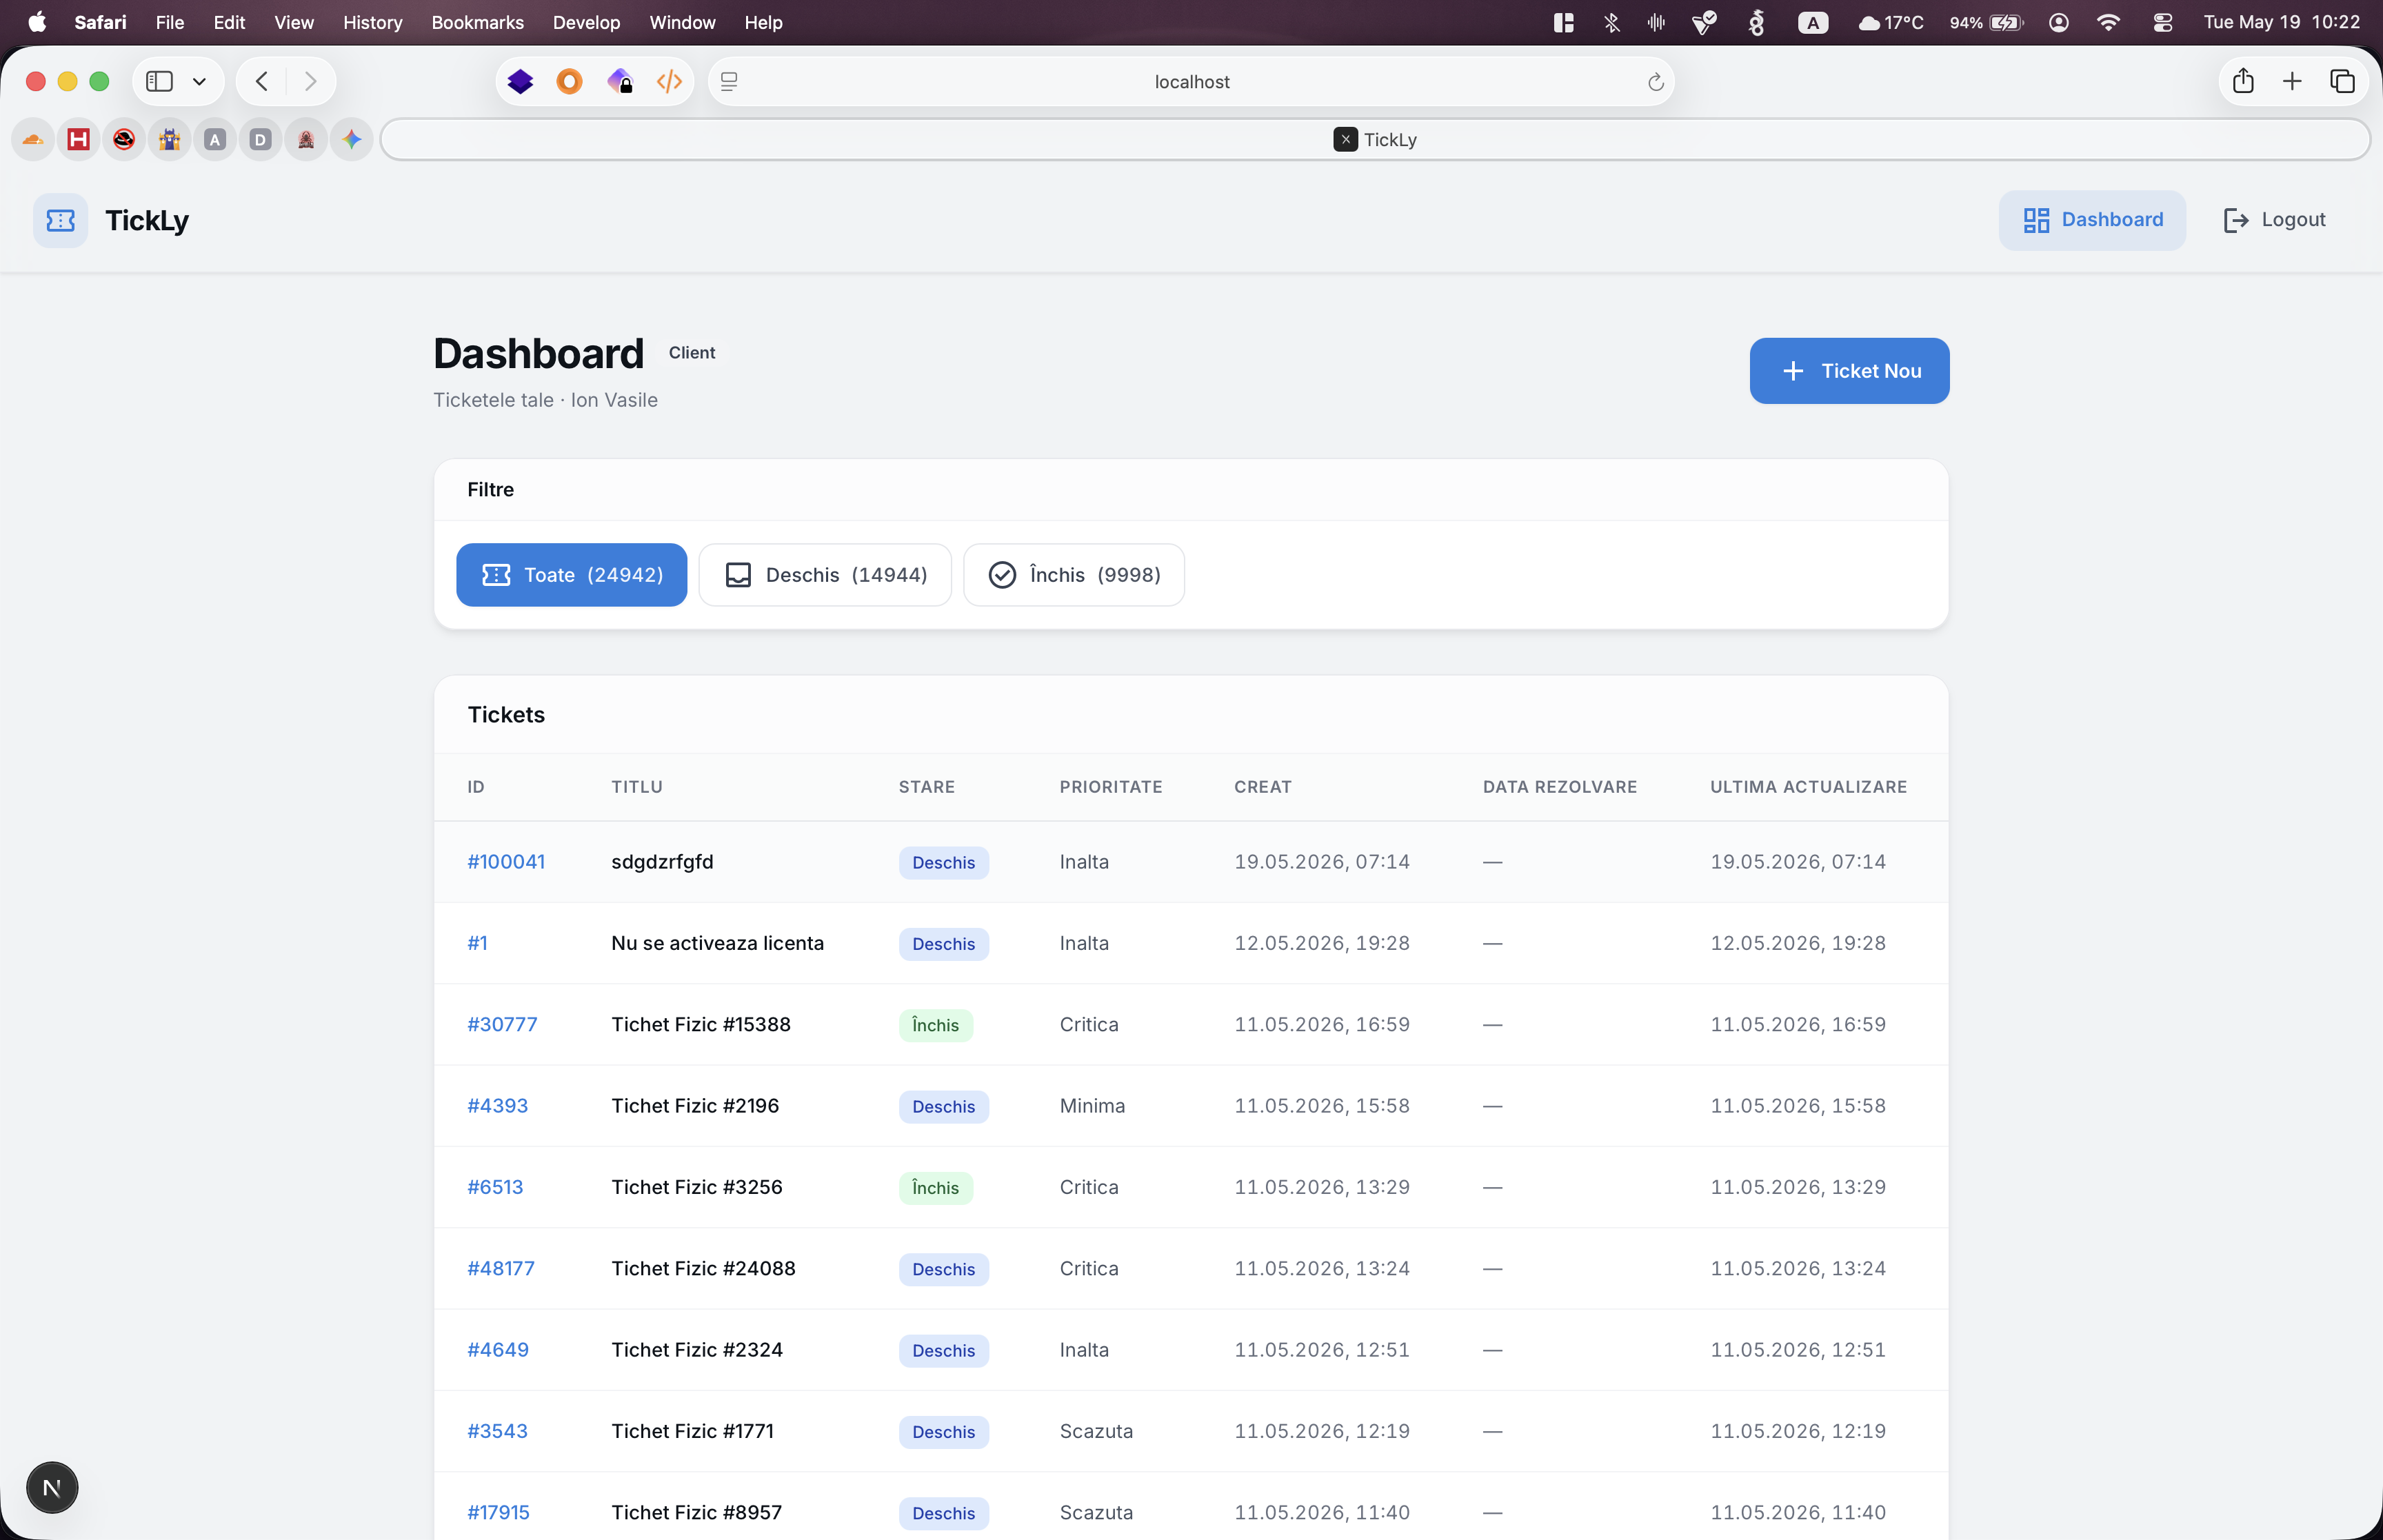
\includegraphics[width=\textwidth]{./assets/app/b2c_module_pt1.png}
        \label{fig:local_view_b2c_1}
    \end{subfigure}
    \hfill
    \begin{subfigure}[b]{0.48\textwidth}
        \centering
        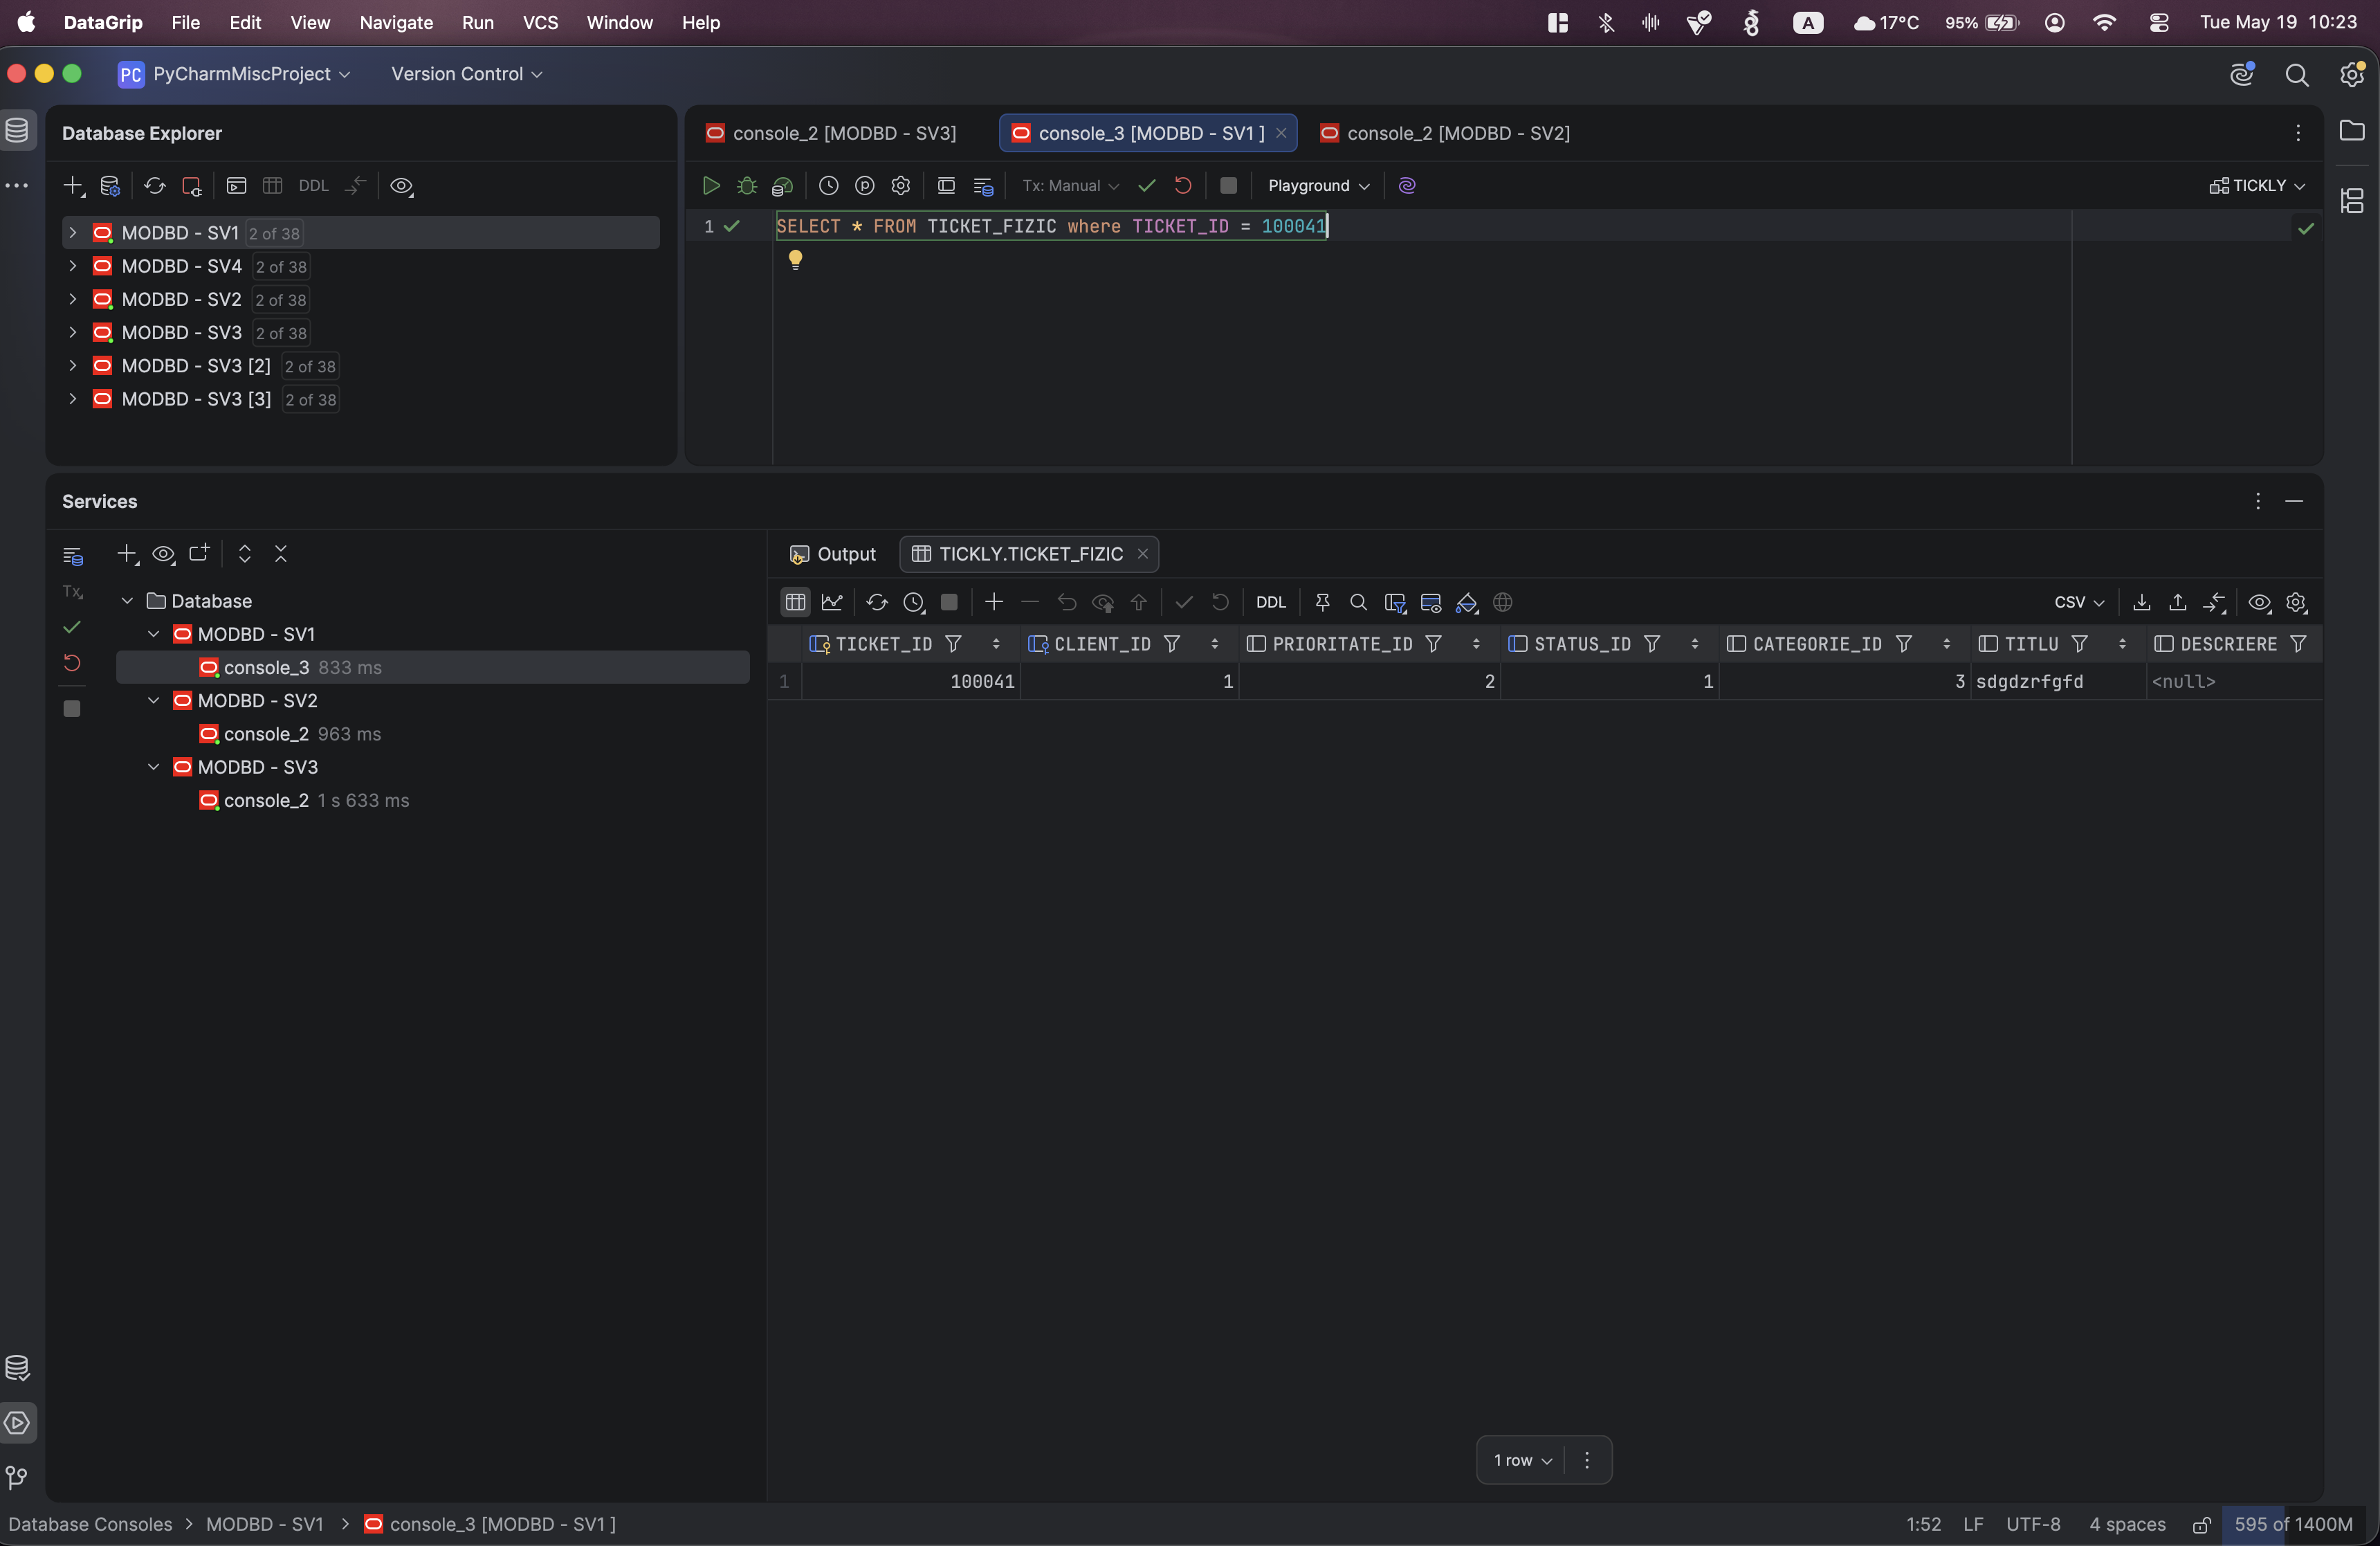
\includegraphics[width=\textwidth]{./assets/app/b2c_module_pt2.png}
        \label{fig:local_view_b2c_2}
    \end{subfigure}
    
    \caption{Local Model B2c}
    \label{fig:dashboard}
\end{figure}

\begin{figure}[H]
    \centering
    \includegraphics[width=0.6\textwidth]{./assets/app/new_ticket.png}
    \caption{New ticket Clients}
    \label{fig:new_tkt}
\end{figure}

\begin{figure}[H]
    \centering
    \includegraphics[width=0.6\textwidth]{./assets/app/ticket.png}
    \caption{Ticket}
    \label{fig:tkt}
\end{figure}